\section{Memory Transaction Optimization}
\label{sec:strategies}

\mypara{Working example.} We take the single-channel 2D convolution example shown in Figure \ref{fig:twostrategies} as a work example to
explain out approach. Here, we slide a $5 \times 5$ filter over a $6 \times 11$ image to produce a $2 \times 7$ output. In this example,
each thread calculates one column of the output. For example, threads 0 and 1 could execute code to slide the filter along the width
dimension. Both threads load two overlapped regions from the input image, thereby generating four duplicate columns. Assume thread 6
demonstrates the process of sliding the filter along the height dimension. It loads two overlapped regions and generates four duplicate
rows.

\mypara{Notations.} Our approach optimizes convolution operations on GPUs by reusing column and row elements. We use following notations
throughout the paper. We use $I$, $F$, and $O$ to represent the input, the filter, and the output respectively, $N$, $C$, $H$, and $W$ to
denote the batch size, the channel, the height, and the width, respectively.

%\begin{table}[t!]
%\centering
%\caption{Notations for the convolution operation.}
%	\begin{tabular}{c|c}
%	\hline
%		$I$, $F$, $O$ & Input, Filter, Output \\
%		\hline
%		$N$, $C$, $H$, $W$ & batch size, channel, height, width\\
%		\hline
%	\end{tabular}
%	\label{tab:notations}
%\end{table}

\subsection{Column Reuse}
\label{sec:creuse}

\begin{figure*}[!t]
\centering
\subfloat[Direct convolution: Each thread loads 5 input elements from global memory.]{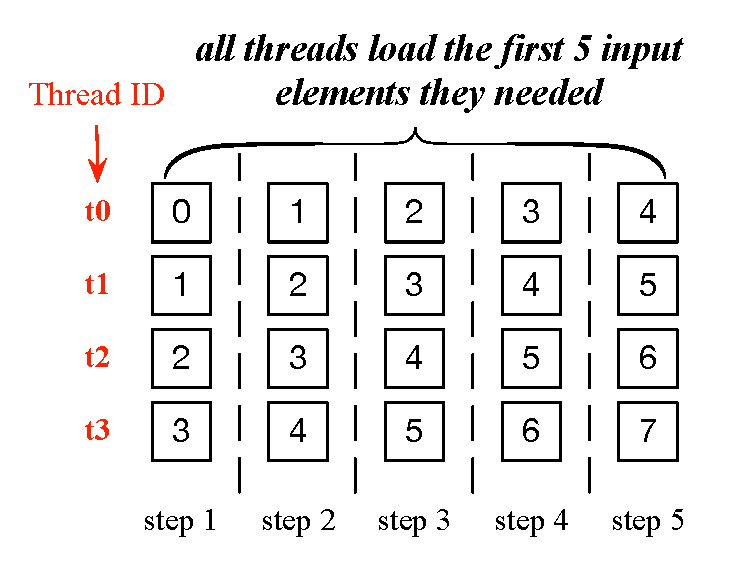
\includegraphics[width=0.32\textwidth,height=4.5cm]{./figure/directconv.eps}
	\label{fig:directalgo}}
\hspace{0em}
\subfloat[Optimized convolution: each thread retrieve its third element from the corresponding thread.]{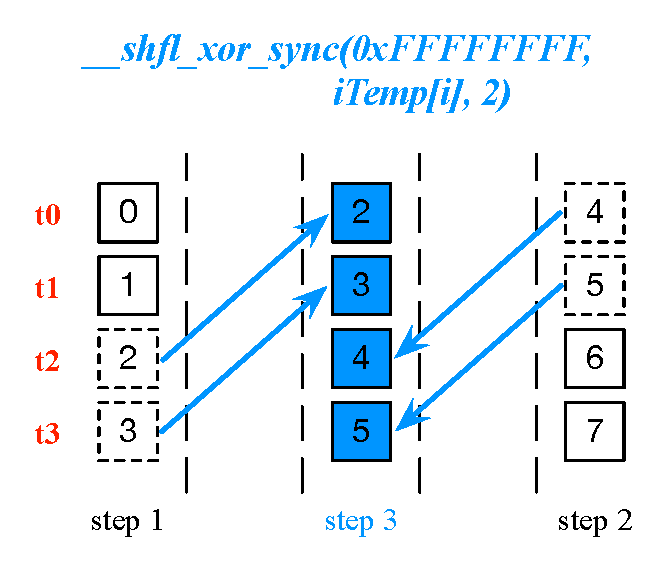
\includegraphics[width=0.32\textwidth,height=4.5cm]{./figure/optalgo1.eps}
	\label{fig:optalgo1}}
\hspace{0em}
\subfloat[Optimized convolution: each thread retrieve its second and fourth elements from corresponding threads.]{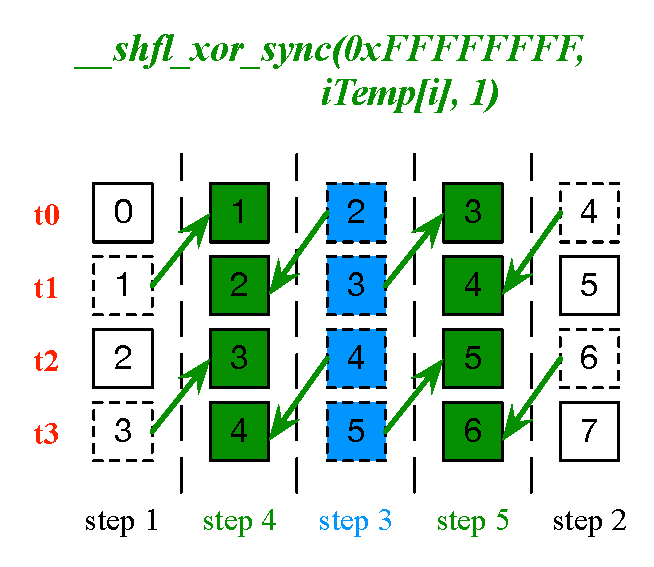
\includegraphics[width=0.32\textwidth,height=4.5cm]{./figure/optalgo2.eps}
	\label{fig:optalgo2}}

\caption{Illustration of direct and optimized convolution. We use a $5 \times 5$ filter  and each thread calculate convolution for one output element. Here we demonstrate how each thread processes first 5 corresponding input elements.}
\label{fig:corealgo}
\end{figure*}



Figure \ref{fig:corealgo} depicts our column reuse algorithm, which consists of a number of steps.

 In step 1 of Figure \ref{fig:directalgo}, each thread loads the first corresponding input elements from the
global memory. Given that the addresses of these elements are contiguous (0, 1, 2, 3), the memory controller can coalesce the accesses into
one memory transaction. Therefore, five memory transactions are required for steps 1-5 of Figure \ref{fig:directalgo}. After completing step 5, each pair of adjacent threads have four
duplicate input elements, which corresponds to the duplicate columns in Figure \ref{fig:twostrategies}.

The input elements 1, 2 and 3 loaded in step 2 would have already been loaded by threads $t1$, $t2$ and $t3$ in step 1 (Figure
\ref{fig:directalgo}). Therefore, we can retrieve the input elements 1, 2 and 3 from the threads $t1$, $t2$ and $t3$ instead of loading
them from the global memory (or L1 cache). This kind of duplication also occurs in steps 3, 4 and 5.

To eliminate the redundant loads, we use the shuffle instructions to exchange input elements among different threads. In steps 1
and 2 of Figure \ref{fig:optalgo1}, each thread loads the corresponding first and fifth input elements from the global memory. In step 3, each
thread utilizes the shuffle instruction to retrieve the third element from another thread. Threads $t0$ and $t1$ retrieve the third elements
from threads $t2$ and $t3$, respectively, and provide the fifth elements (dashed squares in step 2) for both threads.
Similarly, threads $t2$ and $t3$ retrieve the third elements from threads $t0$ and $t1$, respectively, and provide the first
elements (dashed squares in step 1) for threads $t0$ and $t1$. This exchange process can be implemented using the instruction
$shfl\_xor(iTemp[i],2)$ (taking CUDA shuffle as an example, \cite{CUDAtoolkit} provides the exact form of the shuffle instructions), where $iTemp$ is the thread local
array used to store the five input elements, and $i$ indexes which element to provide. For threads $t0$ and $t1$, both need to provide the fifth
elements, thus $i=4$. For threads $t2$ and $t3$, both need to provide the first elements, thus $i=0$.
%The procedure presented in Figure  \ref{fig:optalgo2} is the same as that in Figure \ref{fig:optalgo1}, except that each thread in Figure 3c retrieves the second and fourth elements from its neighboring threads.

However, the instruction $shfl\_xor(iTemp[i],2)$ significantly degrades the performance of the convolution because $iTemp$ is an array with
dynamic indexing, which means that the compiler cannot decide which element to provide at the compile time. Therefore, the compiler
places array $iTemp$ in the local memory, which possesses the same access latency as the global memory, instead of the registers. This process significantly increases the memory access time and degrades the performance of the convolution.

\begin{figure}[t!]
	\centering
	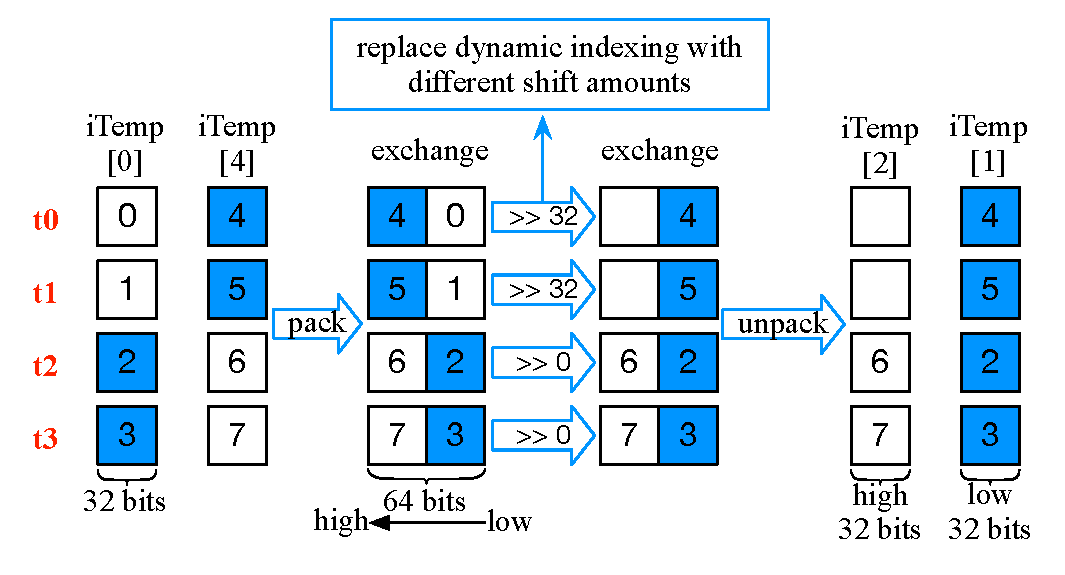
\includegraphics[width=\columnwidth,height=4.5cm]{./figure/exchange.eps}
\caption{Convert the dynamic indexing of array $iTemp$ into static indexing. Therefore, The compiler can put $iTemp$ into registers instead of local memory.}
\label{fig:exchange}
\end{figure}


\begin{algorithm}[t!]
	\KwIn{$iTemp$}
	\KwOut{$iTemp$}
	$tid \gets threadIdx.x$\;
	$mov\ exchange, \{iTemp[0], iTemp[4]\}$\;
	$shift \gets ((tid+2)\&2)<<4$\;
	$exchange \gets exchange >> shift$\;
	$mov\ \{iTemp[1],iTemp[2]\}, exchange$\;
	$iTemp[2] \gets shfl\_xor(iTemp[1],2)$\;	
	
	\caption{RetrieveThirdElement}
	\label{algo:basic}
\end{algorithm}

To convert dynamic indexing into static one, we design Algorithm \ref{algo:basic} for step 3 in Figure \ref{fig:optalgo1} and Algorithm \ref{algo:basic2} for steps 4 and 5 in Figure \ref{fig:optalgo2}. Both algorithms can change dynamic indexing into static indexing and reduce the number of memory accesses. Figure \ref{fig:exchange} illustrates the process of Algorithm \ref{algo:basic}. We first load the corresponding first and fifth input elements into $iTemp$ before passing it to Algorithm \ref{algo:basic}. Then we pack two 32-bit elements into a 64-bit variable $exchange$, where $iTemp[4]$ and $iTemp[0]$ are the high and low 32 bits, respectively (Line 2).  Threads $t0$ and $t1$ must provide their fifth elements, which are the high 32 bits of $exchange$, thus we right shift $exchange$ in both threads by 32 to place $iTemp[4]$ in the low 32 bits. Threads $t2$ and $t3$ must provide their first elements, which are already the low 32 bits of $exchange$. Therefore, we right shift $exchange$ in both threads by 0. The shift amounts of each thread is calculated on the basis of the thread ID (Line 3). Next, unpack $exchange$ into $iTemp[2]$ (high 32 bits) and $iTemp[1]$ (low 32 bits) (Line 5). And $iTemp[1]$ is the element that each thread must provide. Lastly, the shuffle instruction is used to exchange the elements among the threads (Line 6).

\begin{algorithm}[t!]
	\KwIn{$iTemp$}
	\KwOut{$iTemp$}
	$tid \gets threadIdx.x$\;
	$mov\ exchange, \{iTemp[0], iTemp[2]\}$\;
	$shift \gets ((tid+1)\&1)<<5$\;
	$exchange \gets exchange >> shift$\;
	$mov\ \{iTemp[0],iTemp[1]\}, exchange$\;
	$iTemp[1] \gets shfl\_xor(iTemp[0],1)$\;	
	\caption{RetrieveSecondElement}
	\label{algo:basic2}
\end{algorithm}

Algorithm \ref{algo:basic} successfully replace dynamic indexing $i$ in $shfl\_xor(iTemp[i],2)$ with static indexing $1$ in $shfl\_xor(iTemp[1],2)$. {\color{red}And therefore all thread local variables can be put in registers,} which significantly improve the performance of convolution. Steps 4 and 5 in Figure \ref{fig:optalgo2} have similar procedure as step 3 in Figure \ref{fig:optalgo1}. Thus, we slightly modify Algorithm \ref{algo:basic} to obtain Algorithm \ref{algo:basic2}. {\color{red}Other filter sizes can also be handled automatically by our method. For filters of size $3 \times 3$, only Algorithm \ref{algo:basic} is needed to retrieve the second element. For filters of size $7 \times 7$, we consider it as a combination of a $7 \times 5$ filter and a $7 \times 3$ filter with one overlapped column. Then we use Algorithm \ref{algo:basic} and Algorithm \ref{algo:basic2} to retrieve elements for the $7 \times 7$ filter.}

In summary, Algorithms \ref{algo:basic} and Algorithm \ref{algo:basic2} can reduce the number of memory transactions from 5 to 2 and 25 to 10 when 5 and 25 input elements are loaded, respectively. This reduction greatly improves the performance of the convolution.

\subsection{Row Reuse}
\label{sec:rowreuse}
\begin{figure}
	\centering
	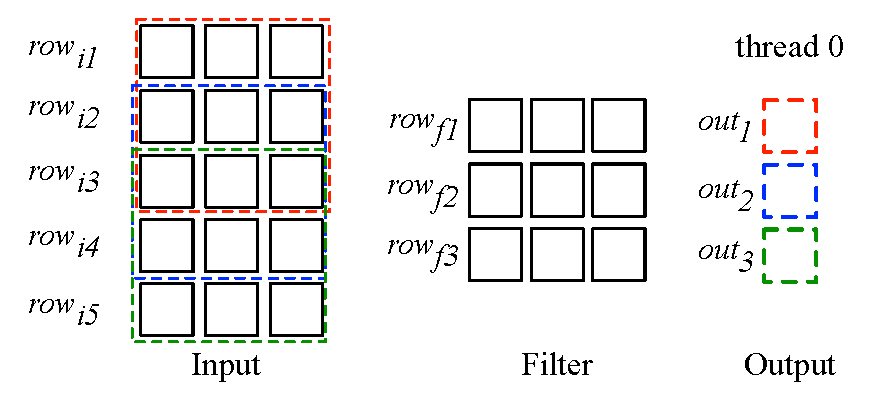
\includegraphics[width=0.9\columnwidth,height=3.7cm]{./figure/rowreuse.eps}
\caption{A $3 \times 3$ filter is used to slide over the input image along height dimension and produce a column of output elements. One thread is used to calculate this column of output elements.}
\label{fig:rowreuse}
\end{figure}

Figure \ref{fig:rowreuse} shows that when sliding the filter over the input image along the height dimension, we can obtain a column of output elements. Our design then uses one thread to calculate one column of output elements. Based on Figure \ref{fig:rowreuse},
we can perform convolution as follows:

\begin{gather*}
  out_0=row_{i0} \cdot row_{f0} + row_{i1} \cdot row_{f1} + row_{i2} \cdot row_{f2} \\
out_{1}=row_{i1} \cdot row_{f0} + row_{i2} \cdot row_{f1} + row_{i3} \cdot row_{f2} \\
out_{2}=row_{i2} \cdot row_{f0} + row_{i3} \cdot row_{f1} + row_{i4} \cdot row_{f2}
\end{gather*}

The above equations suggest that $row_{i1}$ and $row_{i3}$ are loaded twice, and $row_{i2}$ is loaded three times; nine rows should be loaded in total. To eliminate row duplications, we redesign the execution of the convolution. After loading a row from the input, we determine the number of output elements that need the row. For example, $out_0$ needs $row_{i0}$, and $out_0$ and $out_1$ need $row_{i1}$. Then, we use
this row to do inner product with corresponding rows of the filter to calculate the output elements that need this row. The redesigned formulations are shown as follows:
\begin{equation}\nonumber
\begin{aligned}
load\ row_{i0}:
&\ out_0=row_{i0} \cdot row_{f0} \\
load\ row_{i1}:
&\ out_0 = out_0+row_{i1} \cdot row_{f1}\\
&\ out_1=row_{i1} \cdot row_{f0}\\
load\ row_{i2}:
&\ out_0 = out_0+row_{i2} \cdot row_{f2}\\
&\ out_1 = out_1+row_{i2} \cdot row_{f1}\\
&\ out_{2}=row_{i2} \cdot row_{f0}\\
load\ row_{i3}:
&\ out_1=out_1+row_{i3} \cdot row_{f2} \\
&\ out_2=out_2+row_{i3} \cdot row_{f1}\\
load\ row_{i4}:
&\ out_2=out_2+row_{i4} \cdot row_{f2}
\end{aligned}	
\end{equation}



We can see from above equations that only 5 rows are loaded to calculate output elements. {\color{red}Though the number of accesses to $out$ is increased, we store $out$ in registers and the overhead for the increased number of store operations is negligible.} A generalized description of the method is
shown in Algorithm \ref{algo:rowreuse}, where $row$ denotes the row loaded from the input, $index$ denotes the index of $row$, $filter$ denotes
the vector of filter rows and $filter[i]$ means the $i$th row of the filter. Lines 1-5 deal with the first $F_H-1$ rows ($row_{i1}$ and $row_{i2}$ in Figure \ref{algo:rowreuse}), which
are needed by less than $F_H$ output elements. Lines 6-11 deal with the rows that are needed by exact $F_H$ output elements ($row_{i3}$ in
Figure \ref{algo:rowreuse}). Lines 12-17 deal with last $F_H-1$ rows, which are needed by less than $F_H$ output elements ($row_{i4}$
and $row_{i5}$ in Figure \ref{algo:rowreuse}).

\begin{algorithm}
	\KwIn{$row$, $index$, $filter$, $Out$}
	\KwOut{$Out$}
	\If{$index \textless F_H-1$}{
		\For {$i \gets 0$ \KwTo $index+1$}{
			$Out[i] \gets Out[i]+row \cdot filter[index-i]$\;
		}
	}\ElseIf{$index \geq F_H-1$ \textbf{and} $index \textless I_H-F_H+1$}{
		\For {$i \gets 0$ \KwTo $F_H$}{
			$o_{index} \gets index-F_H+1+i$\;
			$Out[o_{index}] \gets Out[o_{index}]+row \cdot filter[F_H-1-i]$\;
		}
	}\Else{
		\For {$i \gets F_H-1$ \KwTo $0$}{
			$o_{index} \gets I_H-F_H+1$\;
			$Out[o_{index}] \gets Out[o_{index}]+row \cdot filter[F_H-i]$\;
		}
	}
	\caption{RowReuse}
	\label{algo:rowreuse}
\end{algorithm}

In summary, Algorithm \ref{algo:rowreuse} eliminates row duplications caused by sliding a filter over the input along height dimension. The
algorithm loads each row of the input exactly once and thus greatly reduces the number of memory transactions.
